\documentclass[12pt,a4paper]{report}

\usepackage{epcc}
\usepackage{graphicx}
\usepackage{listings, listings-rust}
\lstset{
  basicstyle=\footnotesize
}

\begin{document}

%AC%\pagestyle{myheadings}
%AC%\markright{D.~S.~Henty}

%\title{A Latex thesis example}
%\author{D.~S.~Henty}
%\date{\today}

%\maketitle

\pagenumbering{roman}

\title{High Performance Rust}
\author{Jim Walker}
\date{\today}

\makeEPCCtitle

\thispagestyle{empty}

\vspace{12cm}

\begin{center}

\large{MSc in High Performance Computing}

\large{The University of Edinburgh}

\large{Year of Presentation: 2019}

\end{center}

\newpage

\begin{abstract}
This dissertation examines the suitabilty of the Rust programming language, to High Performance Computing (HPC). This examination is made through porting three HPC mini apps to Rust from typical HPC languages and comparing the perfomance of the Rust and the original implementation. We also investigate the readability of Rust's higher level programming syntax for HPC programmers through the use of a questionnaire.
\end{abstract}

\pagenumbering{roman}

\tableofcontents
\listoftables
\listoffigures

\begin{titlepage}
\vspace*{2in}
% an acknowledgements section is completely optional but if you decide
% not to include it you should still include an empty {titlepage}
% environment as this initialises things like section and page numbering.
\section*{Acknowledgements}

This template is a slightly modified version of the one developed by
Prof. Charles Duncan for MSc students in the Dept. of Meteorology. His
acknowledgement follows:

{\em This template has been produced with help from many former students who
have shown different ways of doing things. Please make suggestions for
further improvements.}

\end{titlepage}

\pagenumbering{arabic}

\chapter{Introduction}
In the field of high performance computing, it is difficult to say what is the most popular programming language. Firstly, we must define what we mean by popularity. Do we mean how many CPU hours are spent running programs from a particular language? Or do we mean the languague in which most of the development of new high performance programs is occuring? Or even, do we mean which programming language is most well liked by HPC programmers?
The Rust programming language promises 'High-level ergonomics and low-level control' to help 'you write faster, more reliable software'~\cite{RustBook}.

I think it might be easier to write this section once I know what isn't in it.

\begin{itemize}
    \item The same programming languages have been used in HPC for ages
    \item Maybe we should try something new
    \item Research is a good \& fun thing to do
    \item introducing... Rust! Has proper backing. Seems cool
    \item Let me tell you what I'm gonna tell you, where I'm gonna tell you it, and \textit{why} I'm gonna tell you it
    \item see you at the conclusion!
\end{itemize}

Write about motiviations for questionnaire here.


\chapter{Background}
\section{Parallel Programming Languages for HPC}
HPC (High Perfomrance Computing) refers to computation performed on supercomputers. 
Supercomputers generally have more and faster cores than personal computers. They are normally networked together with fast interconnect to allow for high data throughput, and are used for highly numerical scientific programs.
To fully leverage the potential of these supercomputers many computing cores, programmers use parallel computing techniques, in programming languages which run as fast as possible on the hardware.

The three main languages used in HPC are Fortran, C and C++. They are all well established within the field, as shown by table~\ref{tab:langs}, which shows the proportion of compute time taken up by these languages on Archer, (Advanced Research Computing High End Resource), one of the UK's primary academic research supercomputers.
Whilst Fortran takes up the majority of compute time on Archer, this dissertation will focus on C and C++, as they are more comparable to Rust (their similarities are discussed further in the next sections).

\begin{table}[h]
  \centering
  \begin{tabular}{|c|c|}
    \hline
    & \textbf{ARCHER} \\
    \hline
    Fortran & 69.3\% \\
    \hline
    C++ & 7.4\% \\
    \hline
    C & 6.3\% \\
    \hline
    Unidentified & 19.4\% \\
    \hline
  \end{tabular}
  \caption{Breakdown of CPU usage by programming language~\cite{Turner2015}}
  \label{tab:langs}
\end{table}

There are two central paradigms to parallel computing, message passing parallelism and share memory parallelism. In message passing parallelism, processes work on private data, and share data by sending and receiving messages. This form of parallelism is very scalable, and can run on geographically distributed heteregenous nodes~\cite{SETI}. Examples of message passing parallelism include the MPI (message passing interface) standard, and Go's channels.

Shared memory parallelism, by comparison, has processes that share access to a region of memory. Whilst programs using can run on multiple nodes through technologies like PGAS (Partitioned Globabl Address Space)\todo{does this count?}, these nodes are still normally required to be homogenous. Shared memory parallelism is most effective when it runs on a single node with many processing cores. Although this paradigm has recently grown in usage through the usage of many core architures on GPUs, this dissertation will concern itself with shared memory parallelism, due to Rust's interesting shared memory model. Whilst shared memory parallelism is a fast way to write and run programs, there are difficulties inherint in implementing this technique in languages like C and C++ that are not memory safe. In the next section, I will discuss these difficulties.

\section{C and C++}
The C programming language was developed in 1972, as a `system implementation language'~\cite{Ritchie:1993}. Its first purpose was to program the UNIX operating systems and the utilities which were fundamental to its use, like \texttt{cat} and \texttt{rm}. Since that point, the C programming language has always been associated with low level computing. In this case, low level computing means computing which is able to be compiled to very efficient machine code, and gives the programmer fine grained memory management.

Today, the Linux kernel, which provides the foundation for the operating systems used on the vast majority of the world's supercomputers, is 96\% written in C~\cite{LinuxKernel}. Many of the programs that are run on these supercomputers are written in C~\cite{fftw, ffs, foam}

Despite C's success, only seven years after it was first developed, Bjarne Stroustrup began working on an extended version of C, which was to become C++. In 1985, the first commercial edition of C++ was released~\cite{CPPFAQS}. Two of C++'s most notable extensions to C are the introduction of classes, to allow for object oriented programming, and templates, which allow for generic programming. C++ also uses a stronger type system than C, which prevents bugs caused by implicit conversion.

Like C, the design of C++ focused on system programming~\cite{CplusEssence}, and like C, it has become a common language of choice for developing HPC codes~\cite{foam}\todo{more examples here}, a fact which is helped by the close similarity of the two languages. Many C programs are valid C++ programs. C and C++ are also considered two of the languages which, when compiled, run fastest.

The speed of C and C++ is one of their most celebrated design features. However, there are other, less positive consequences of the design of these two languages, which require programmers to use them with care. This dissertation is principally concerned with the memory safety issues of C and C++, which can cause programs to crash, or return incorrect data.

Listing~\ref{lst:use-free} demonstrates one of the C and C++'s memory pitfalls, known as use after free. The code rs valid C and C++. Use after free occurs when a program attempts to use a section of memory after it has been released back to the operating system.
The freeing of \texttt{array} here means that the contents of it cannot be guaranteed when it is printed.

\begin{code}
\begin{minted}{c}
#include <stdio.h>
#include <stdlib.h>

int main(){
    int* array = (int*) malloc(sizeof(int)*10);
    for (int i=0; i<10; i++){
        array[i] = i;
    }
    free(array);
    printf("%d\n", array[1]);
    return 1;
}
\end{minted}
\captionof{listing}{C and C++: Use after free}
\label{lst:use-free}
\end{code}

In larger programs, this can lead to calculations being made using incorrect data, which has been overwritten by the operating system, or another thread from the same program. Other common sequential memory pitfalls in C and C++ are:

\begin{itemize}
    \item \textbf{Double Free:} Attempting to free memory which has already been freed can lead to undefined behaviour.
    \item \textbf{Heap Exhaustion:} The program tries to allocate more memory than the amount available. This can be the result of a memory leak, when data is not always freed after being allocated.
    \item \textbf{Buffer Overrun:} Attempting to access the $n^{th}$ element of an array which is only of length $n$. This can lead to the reading incorrect data, or accidentally trashing other memory within the same program.
    \item \textbf{Data Race:} This type of non-deterministic bug occurs when two or more threads need to update a variable, but the outcome of this update depends on the timing of the threads accessing the variable. An example of a data race is given in listing~\ref{lst:omp-eg}.
\end{itemize}

Whilst it is possible to write memory safe code with memory unsafe languages, it is hard to do so. It is impossible to know how exactly many bugs exist in HPC codes,and to know how many of those are caused by memory safety issues.
As an indication, we can take data from Microsoft, which shows that 70\% of their Common Vulnerabilities and Exposures (CVEs) are caused by memory safety issues~\cite{MicroBugs}. There is no good estimate of the amount of memory safety errors that exist in C or C++ HPC programs, but if we take the Microsoft data to be indicative of general error sources, then the lack of memory safety in C and C++ should be a cause of concern for HPC programmers.

\subsection{OpenMP}
The first specification for the OpenMP (Open Multi-Processing) Fortran, C and C++ application program interface (API) was released in October 1998. Its aim was to `allow users to create and manage parallel programs while permitting portability'~\cite{OpenMPSpec}. It acts as an extension to the C and C++ language specifications, leaving responsibility for implementing it to compiler writers, just as with C and C++. New specifications of OpenMP are periodically released, and it is now recognised as a cornerstone of HPC, as can be seen from the large number of people who sit on the its Architecture Review Board~\cite{OpenMPARB}.

OpenMP's parallelism model is based around shared memory parallelism. This is done to reflect the reality of the multi-core hardware which are used in HPC\@. Multi-core processors share memory with each other, and each core can access any memory address on that node.  

An example OpenMP program is shown in listing~\ref{lst:omp-eg}. It is valid C and C++. A key feature of OpenMP are its \texttt{\#pragma omp} statements, which issue parallelism related directives to the compiler. 
One of OpenMP's core strengths is its succinct abstractions to the underlying threading API, irrespective of the platform it's running on. Here, there \texttt{\#pragma omp} statement signifies the part of the code to be parallelised, and importantly, does not do so at the cost of obscuring the programs serial intent.
The example parallelises the for loop, and sets the number of threads through the OMP\_NUM\_THREADS environment variable. In this program, the variable \texttt{a} is set to zero, and it is then incremented in the for loop.

\begin{code}
\begin{minted}{c}
#include <omp.h>
#include <stdio.h>
int main(){
    int a = 0;
    #pragma omp parallel for
    for (int i=0; i<10; i++){
        a++;
    }
    printf("%d\n", a);
    return 0;
}
\end{minted}
\captionof{listing}{C and C++: OpenMP Data Race}
\label{lst:omp-eg}
\end{code}

However, the output of this program in non-deterministic, as it includes a data race condition. If the main thread completes first, it will print the value of \texttt{a} that currently exists, not wait until all the other threads have completed. 

This race condition leads to different values being printed by the program on different executions. To solve this problem, a \texttt{\#pragma omp barrier} statement must be inserted at the end of the for loop. As with the other memory errors mentioned earlier however, these mistakes are not always found before using a program.

\section{Rust}\label{sec:rust}
The Rust programming language was started life as a side project by an employee of the Mozilla foundation, before becoming adopted and launched by it in 2011~\cite{FutureTense}. Rust's design was stated to be an `Unapologetic interest in the static, structured, concurrent, large-systems language niche'~\cite{pServo}. Like C and C++, Rust's early design aims included a the goal of becoming a systems language. Rust like C has structs, and shares behaviours between structs through composition with traits, but not with inheritence, like C++.

Rust's initial design ideas mainly diverge from C and C++ in its aims to provide the programmer with memory safety. Two ideas, immutability and ownership are used to achieve this improvement. 

Ownership is one of Rust's best known features. It `allows Rust to be completely memory-safe'~\cite{NomOwner}, and works by using the compiler's borrow checker to ensure that Rust's ownership model is satisfied by a given program before compiling it.

In listing~\ref{lst:rust-free} we present a Rust program that does not satisfy the ownership model, and therefore does not compile. The first line of the main function heap allocates memory to a vector of 10 elements, and gives each element a value of four. This vector is labelled \texttt{vector}. It is created using a macro, which is similar to functions in Rust, except that they can take a variable number of arguments, formatted in different ways, like with semi-colons.

\begin{code}
\begin{minted}{rust}
fn main(){
    let vector = vec![4;10];
    drop(vector);
    println!("{}", vector[2]);
}
\end{minted}
\captionof{listing}{Rust: Use after free}
\label{lst:rust-free}
\end{code}

The \texttt{drop()} function is then called on the vector, which is similar to \texttt{free()}. \texttt{drop()} is automatically called on values when they go out of scope. It is more accurate to think of \texttt{drop()} as something akin to C++'s destructors, but both those and this function do, at their core, release memory back to the operating system. However, attempting to use a variable after it has been dropped is illegal in Rust, resulting in the error message below:

\begin{code}
\begin{minted}{bash}
error[E0382]: borrow of moved value: 'array'
 --> src/main.rs:6:20
  |
2 |     let vector = vec![4;10];
  |         ----- move occurs because 'array' has type 'std::vec::Vec<i32>',
  which does not implement the 'Copy' trait
3 |     drop(vector);
  |          ----- value moved here
...
6 |     println!("{}", vector[2]);
  |                    ^^^^^ value borrowed here after move

error: aborting due to previous error
\end{minted}
\captionof{listing}{Rust Compiler: Use after free}
\label{lst:rust-borrow-move}
\end{code}

This is rust's borrow checker complaining that the program does not follow the ownership model. When the value of \texttt{vector} is dropped, in the Rust ownership model, the ownership of \texttt{vector} is moved into the drop function, and is not returned. When the program later tries to use (borrow) the variable, it is therefore unable to, as Rust only allows for values to have one owner at a time.


Allowing values to only have one owner at a time is worked around by functions borrowing mutable or immutable references to those variables. For example, if a function needs to mutate a vector, it will need to specify that type in it's function arguments, i.e. \texttt{v: \&mut Vec<i32>}, v where v is of the type of a borrowed mutable reference to a vector containing 32 bit integers.
This requirement also highlights how Rust's borrow checker is reinforced by a strong type system, which requires the function parameter to be of a certain type, and immutability by default, which makes it explicit which functions will change values that are passed to them.

Memory safety is further improved in Rust by the absence of null pointers through the use of optional values. If a function may return something or nothing, it returns an \texttt{Option<T>}, which can either be \texttt{Some(v)} where \texttt{v} is a value of type \texttt{T}, or \texttt{None}. Pattern matching can be used to succinctly unwrap these variables.

Rust also makes the promise that it is free of data races, with certain caveats. Data races are defined as:
\begin{itemize}
    \item `two or more threads concurrently accessing a location of memory
    \item one of them is a write
    \item one of them is unsynchronized'
\end{itemize}
\begin{flushright}
--- The Rustonomicon: Data Races and Race Conditions~\cite{NomRace}
\end{flushright}

and are only absent from safe rust. This does not mean that Rust prevents programmers from creating deadlock situations entirely, only that a certain subsection of data races are prevented, and only in safe Rust. Unsafe Rust exists as another language within Rust, delimited within \texttt{unsafe} blocks. It exists because there a limits to such a safe Rust which do not accurately reflect the underlying hardware on which it runs. However, it is not seen as being the `\textit{true} Rust Programming Language'~\cite{NomSafe}, and therefore this dissertation will only examine safe Rust. I will also attempt to write Rust in an idiomatic style in attempt to write Rust which is as representative of Rust as possible. Idiomatic Rust tends to chain function calls and use pattern matching to achieve more succinct code.

Unlike C and C++, Rust comes with a build tool and dependency manager, Cargo, which wraps around the Rust compiler. Cargo allows users to specify a programs dependencies, which are automatically downloaded and integrated into that program from external repositories. In Rust, these dependencies are called crates. In this dissertation, I make extensive use of the Rayon crate, as explained in section~\ref{sec:back-rayon}.

Some work has been done to investigate the applicability of Rust to HPC~\todo{citations here}, but it expertise in the language is still low within the community~\todo{cite maybe?}. As such, I will gain technical support from the Rust community through the official subreddit and community discord channels when I encounter a problem particular to Rust.

\subsection{Rayon}\label{sec:back-rayon}
Rayon is the one of the most popular crates for parallelism in Rust, and features heavily in the Rust cookbook~\cite{RustCookPara}. In a fashion similar to OpenMP, it abstracts complicated underlying threading technologies. Unlike OpenMP, Rayon concentrates on parallel iterators, and like Rust promises data race freedom.

Rayon's parallel iterators are conceptually descended from Rust's sequential iterators. An iterator is a function which provides access to the elements of a collection, so that an operation can be performed on a set of those elements. In Rust, iterators implement the Iterator trait, which provides access to the current item, and a \texttt{next()} function, which returns an optional value. An example of a sequential iterator is shown in listing~\ref{lst:rust-seq-iter}, where a vector of 5 elements, each with value 2, are first each multiplied by five in the \texttt{map()} function, using an anonymous function. In Rust, these are called closures. The \texttt{fold()} function then returns the product of all the elements in the mapped collection, which is 10000. The first argument of fold provides the identity value for the fold, which is used to begin the operation.

Rayon's parallel iterators work in a similar way to Rust's sequential iterators, except that they give sections of the iterable collection to separate threads to calculate. The parallel iterator methods also have slightly different syntax, as demonstrated by listing~\ref{lst:rust-par-iter}. This listing produces the same result as~\ref{lst:rust-seq-iter}, but the \texttt{fold()} is different.

\noindent\begin{minipage}{.49\textwidth}
\begin{code}
\begin{minted}{rust}
fn main(){
  let v = vec![2;5];
  let s = v.iter()
           .map(|x| x * 5)
           .fold(1, |acc, x| acc * x);
  println!("{}", s);
}
\end{minted}
\captionof{listing}{Rust: sequential iterator}
\label{lst:rust-seq-iter}
\end{code}
\end{minipage}\hfill
\begin{minipage}{.49\textwidth}
\begin{code}
\begin{minted}[fontsize=\scriptsize]{rust}
extern crate rayon;
use rayon::prelude::*;

fn main(){
  let v = vec![2;5];
  let s = v.par_iter()
           .fold(|| 5, |acc, x| acc * x)
           .reduce(|| 1, |x, y| x * y);
  println!("{}", s);
}
\end{minted}
\captionof{listing}{Rayon: parallel iterator}
\label{lst:rust-par-iter}
\label{lst:iters-a}
\end{code}
\end{minipage}

The first argument to the parallel \texttt{fold()} is an identity closure, which generates the identity value. This is done so that the different threads can have their own copy of the identity value. The output of the fold is different too, as each thread performs a fold on its section, and therefore does not return a single value. A parallel reduction is called on the resulting collection, which delivers the product of all the values left in the collection.
In this way, the fold reduce pattern is `roughly equivalent to map reduce'~\cite{rayonFold} in effect. It is also noteworthy that \texttt{par\_iter()} uses a number of threads set by the environment variable RAYON\_NUM\_THREADS, which is similar to OpenMP\@.

Iterators are safer than for loops. They prevent threads trying to access data beyond array boundaries, without a performance cost. However, they do lack of flexibility compared to for loops. From within a for loop, the programmer can access the $i^{th}$ element of the collection they are iterating over, or the $i-1^{th}$ element, if they choose to through simple index arithmetic. I will investigate the costs and the benefit of this trade off in my dissertation.

\section{Kernels}
In Computing a Kernel is often used to describe a part of a larger program that is responisble for much of that programs execution time. Within the context of this dissertation however, I will use kernel to describe the whole of a very small program, which is itself representative of a common HPC task. In this way, my usage of kernels is similar to how Mini-apps have been used in research in the past.

Mini-apps are a well established method of assessing new programming languages or techniques within HPC~\cite{Mallinson:2014, Slaughter:2015, martineau2017arch}. A mini-app is a small program which reproduces some functionality of a common HPC use case. Often, the program will be implemented using one particular technology, and then ported to another technology. The performance of the two mini-apps will then be tested, to see which technology is better suited to the particular problem represented by that mini-app. Such an approach gives quantitative data which provides a strong indication for the performance of a technology in a full implementation of an application. 
This dissertation will follow a similar approach of evaluating a program through the performance of a kernel, using the test data to find any weaknesses in the Rust or original implementation.

I am going to use Kernels rather than mini-apps because mini apps often focus on a particular scientific domain, whilst performing the same sort of calculations. For example, a meterogical mini-app and a fluid dynamics mini-app might both use the jacobi method~\cite{muller2014, schippers1982}, but only differ in their input and preconditioning of data.
Through only attempting to port the core part of a program, this dissertation will be able to examine a breadth of use case scenarios, hopefully without losing any of the depth of examining mini-apps.

I will also evaluate the ease with which I am able to port a kernel into Rust. These observations will provide insight into what it is like to program in Rust, if its strict memory model and functional idioms help or hinder translation from the imperative languages which the ported programs are written in. This qualitative, partly experiential information will hopefully provide an insight into the actual practicalities of programming in Rust. For Rust to be fully accepted by the HPC community, it is necessary that the program fulfils the functional requirements of speed and scaling, alongside non functional requirements, of usability and user experience. The first factor provides a reason for using Rust programs in HPC, the second provides an impetus for learning how to write those programs.

I will use reference implementations of the kernels that have already been written by other people rather than writing my own. I will do this for two reason. Firstly, a more fairer comparison between Rust and C or C++ can be made if I do not write the original implementation myself, so that my lack of knowledge in one of the programs makes it perform worser. Secondly, by selectin reference implemetations that have already been written, I can save time and not write them myself, allowing me a deeper investiagation of the Rust implementations.
\section{Roofline} stuff makes sense here.


\chapter{Methodology}
\section{Kernel Selection}
So that a breadth of usage scenarios were examined, three kernels were selected based on their conformity to the following set of criteria.
\begin{itemize}
  \item \textbf{The part of the program responsible for more than two thirds of the processing time should not be more than 1500 lines.} To ensure that I fully implemented three ports of existing kernels, it was necessary to limit the size of the kernels that could be considered. This was an unfortunately necessary decision to make. Whilst it reduced the field of possible kernels, it helpfully excluded any overly complex mini-apps.

  \item \textbf{The program must use shared memory parallelism and target the CPU.} Rust's (supposed) zero cost memory safety features are its differentiating factor. The best way to test the true cost of Rust's memory safety features would be through shared memory parallelism, where a poor implementation of memory management will make itself evident through poor performance. Programs which target the GPU rather than the CPU will not be considered, as the current implementations for Rust to target GPUs involve calling out to existing GPU APIs. Therefore, any analysis of a Rust program targeting a GPU would largely be an analysis of the GPU API itself.

  \item \textbf{The program run time should reasonably decrease as the number of threads increases, at least until the number of threads reaches 32.} It is important that any kernel considered is capable of scaling to the high core counts normally seen in HPC.I will be running the kernels on Cirrus, which supports 36 real threads.

  \item \textbf{The program operate on data greater than the CPU's L3 Cache} so that we can be sure that the kernel is representative of working on large data sets. Cirrus has an L3 cache of 45MiB. As each node has 256GB of RAM, a central constraint when working with large data sets is the speed with which data is loaded into the cache. Speed is often achieved by programs in this area through vectorisation, the use of which can be deduced from a program's assembly code. If there is a large performance difference between Rust and the reference kernels, we can use the program's assembly code to reason about that difference.

  \item \textbf{The program must be written in C or C++.} This restriction allows us to choose work which is more representative of HPC programs that actually run on HPC systems, rather than python programs which call out to pre-compiled libraries. Unlike Fortran, C and C++ use array indexing and layout conventions similar to Rust, which will make porting programs from them easier.

  \item \textbf{The program must use OMP.} This is a typical approach for shared memory parallelism in HPC\@. Use of a library to do the parallel processing also further standardises the candidate programs, which will lead to a deeper understanding of the kernel's performance factors.
\end{itemize}

I used this selection criteria to compile a long list of potential kernels to port to Rust. From this long list, I selected the Babel Stream, sparse matrix vector multiplication and K-means clustering.

\subsection{Babel Stream}

Babel Stream is a memory bench marking tool which was developed by the university of Bristol. Babel Stream was written to primarily target GPUs, but it is able to target CPUs too~\cite{BabelStream}.  It is written in C++, supports OpenMP and allows one to set the problem size when executing the program, so we can be sure we exceed the size of L3 cache. Tests found the kernel to scale well, and although the program as a whole is quite large, when one ignores parallel technologies excluded by our selection criteria, the amount of code which needs to be ported to Rust falls well within our bounds. I found Babel Stream easy to install and run, and initial testing showed us that the program scaled well.

Babel Stream performs simple operations on three arrays of either 32 or 64 bit floating point numbers, $a$, $b$ and $c$. The values of $a$ are set to 0.1, $b$'s to 0.2, and $c$'s to 0.0. Stream performs five operations $n$ times on the arrays, where $n$ is a specified command line argument. The operations are listed below:
\begin{itemize}
  \item \textbf{Copy:} Data is copied from the array $a$ into array $c$
  \item \textbf{Multiply:} Data in $c$ is multiplied by a scalar and stored in $b$
  \item \textbf{Add:} The values in $a$ and $b$ are added together and stored in $c$
  \item \textbf{Triad:} The program then multiplies the new values in $c$ by the same scalar value, adds it to $b$ and stores the value in $a$
  \item \textbf{Dot:} The dot product is performed on arrays $a$ and $b$. This is when every nth element of $a$ is multiplied by the nth element of $b$, and summed.
\end{itemize}
The resulting values in the arrays are then compared against separately calculated reference values, and examined to see if their average error is greater than that number types epsilon value.

Babel Stream's operations are `\textit{memory bandwidth bound}'~\cite{BabelStream}, because they are so simple. Therefore, when implemented through different technologies, Babel Stream provides an insight into the memory bandwidth of that technology, and gives an indication of how the design choices of that technology influences its performance.

\subsection{Sparse Matrix Vector Multiplication}

The Sparse Kernel~\cite{ParResSparse} forms part of the Parallel Research Kernels suite, developed by the Parallel Research Tools group. Sparse matrix vector multiplication (SpMV) is a common HPC operation, used to solve a broad range of scientific problems~\cite{Sedaghati:2015, spMVGPU, DBLP:journals}.

The kernel mostly one file, sparse.c, which in total is 353 lines of code. The implementation is in C and OpenMP, and tests found it to scale to a high thread count. As with Babel Stream, the program allows one to set problem size through command line arguments, allowing us to ensure the program operated on data greater than the CPU's L3 cache.

In the selection process, I found that the programs lack of dependencies made it easy to install and run, and that it scaled well.

The program represents its sparse matrix through the compressed sparse row (CSR) format. This format uses key information about the matrix to avoid storing all of the sparse matrix's redundant zeros in the computer's memory. The information used to do this are the number of rows and columns the matrix has, and the number of non zero values which exist in the matrix. These three values are used to build three vectors, one holding all the non zero values of the matrix, another vector of the same length holding the column indexes for all of those values, in order, and lastly a smaller vector which holds the index at which a particular row starts. For example, if we wanted the element at 24,32 within the vector, we would look in the 24\textsuperscript{th} element of the row start vector, which would give us the y index of the element. If this did not match the y index we were looking for, in this case 32, we would then look at the next element until we found it. Once we have found the element, we can get the value from the value vector using the index we construct from adding the 24\textsuperscript{th} element of the row start vector, added to however many times we needed to look at the next value to before we found the appropriate y index.

The particular implementation of SpMV which we are porting to Rust uses a user defined grid size, over which a user defined periodic stencil is applied to find the number of non zero entries. The implementation parallelises its initialisation and the actual multiplication of the values using simple \texttt{\#pragma} statements.

This kernel will hopefully provide a realistic idea of how well Rust can perform one of the most common HPC operations.

\subsection{K-Means clustering}

K-means clustering is a `process for partitioning an $N$-dimensional population into $K$ sets'~\cite{macqueen1967}, where the number of sets is less than $N$, and each set of is clustered around a local mean. K-means clustering finds many uses in HPC, particularly in data analysis~\cite{DBLP:journals/corr/ChakrabortyND14a, ordovas2014fast}, and is so ubiquitous throughout HPC that implementations of it are already used to evaluate software and hardware~\cite{Yang2014}.

My reference implementation for this code comes from Jaiwei Zhuang's CS205 project~\cite{CS205}. It is written in C and uses OPENMP, and is less than 200 lines long. The data processed by the program can be generated by a script, allowing us to work on an arbitrary amount of data. The kernel is written so that all processing is done by the CPU\@. It is of particular interest to us that the kernel reads its data from a NetCDF file, which is common in HPC\@. The code is well documented and concise.

After the Kernel has read in the program data, it performs the clustering process. It does this by first filling the \texttt{old\_cluster\_centres} array with random data, and then beginning its central processing loop.
\begin{itemize}
  \item \textbf{Expectation:} Assign population points to their nearest cluster centre, by looping over every member of the population, and finding the minimum distance between that point all the cluster centres. At this stage, the minimum distances found between the population points and their cluster centres is also found. This is the stage which is parallelises.
  \item \textbf{Maximisation:} Next, the cluster centres are set to the mean, which is calculated in two steps.
  \begin{itemize}
    \item \textbf{1:} The size of the cluster is calculated by looping over every point and finding its cluster centre, and then incriminating that cluster centres population count. The sum of the points in that cluster is also calculated and stored in the \texttt{new\_cluster\_centres} array.
   \item \textbf{2:} The sum of the cluster is divided by the size of it, and stored in to the \texttt{old\_cluster\_centres} for use on the next iteration of the loop.
   \end{itemize}
\end{itemize}
This loop continues until it reaches a pre defined maximum iteration value, or the sum of the minimum distance values becomes less than a certain tolerance value. The program then writes data back out to the NetCDF file it read the data from originally.

I found this program quite difficult to install and run due to the NetCDF dependency. My first attempt to install NetCDF through the script included in the repository ended with me unable to boot into my laptop. Subsequent attempts to install NetCDF through package managers were also not successful, although they were less damaging to my system. To compile the kernel on cirrus I had to make sure I had selected the correct combination of NetCDF and HDF5 library versions, mostly through guest work. However, once I had accomplished this task, compiling the program itself was easy. The kernel then showed itself to be able to scale adequately enough for the interests of this project.
\section{Implementation}
Implementation of all three programs followed the same process, as outlined in Figure~\ref{fig:imp-flow}. The full process would take between three to four weeks to complete for each kernel. I first implemented Babel Stream, then the sparse matrix multiplication kernel and finally the K means kernel, in that order.

\begin{figure}
  \center
  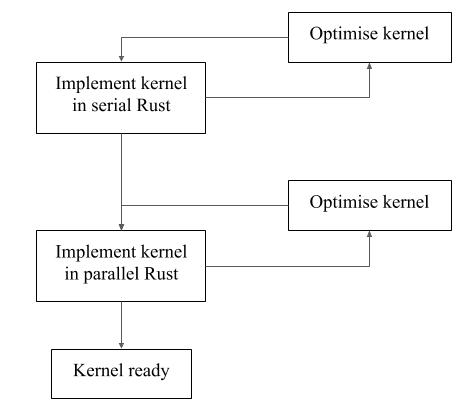
\includegraphics[height=8cm]{figs/ImplementationFlow.png}
  \caption{Flow Diagram for Implementation Process}
  \label{fig:imp-flow}
\end{figure}

\subsection{Porting to Serial Rust}
Once a candidate kernel is selected, it is implemented in Rust in serial. Any differences between the  behaviour of the Rust and the original implementation are thought of as bugs, and are eradicated or minimised as far as is possible. For ease of development, the Rust crate Clap was used to read command line arguments for the program, leading to Rust implementations of kernels being called with slightly different syntax. This difference was deemed to be superficial enough to be allowable. Kernel output was ensured to be as similar as possible to aid data-collection from both implementations.

Babel Stream was in some ways one of the hardest to Kernels to port to serial Rust. This was partly due to it being the first program which I attempted to port, but also because of Rusts type system and the use of generics. The original C++ implementation of the program uses templates to allow the user to choose to use 32 or 64 bit floating numbers when running the program. To achieve the same thing in Rust, generic types have to be used, which are defined through traits.

I found that using generics in Rust made reading error messages slightly difficult, but easier to parse once the offending code was removed into a smaller example, and stripped of its generic type. Generics in Rust necessitate slightly cumbersome syntax, for example, \texttt{T::from(0).unwrap()} is used to generate a zero of type T. This expression generates an option type, which in this case is \texttt{Some(0.0)}, and is then unwrapped into simply \texttt{0.0}. Rust does this to allow programmers to deal with cases where a value of type T is impossible to generate from the input value, such as casting a value greater than $2^{32} - 1$ to a signed 32 bit value. In this circumstance, the value returned would be \texttt{None}, which the programmer would then have to deal with. As zero can always be successfully cast to a 32 or 64 bit floating point number, it is safe to simply unwrap the value here, but if it was a number that could not be cast to the type, then the program would crash at this point. A C or C++ program doing the same thing would not crash, but its result would be undefined. \todo{should I discuss the design choices made here, and their implications for Rust in HPC}

The Rust implementation of Babel stream, like the reference implementation, creates a stream object which calls certain functions on its own data sets. This was quite easy to implement as Rust has enough features of object oriented design, such as allowing objects to contain data and behaviour for these simple objects to work. However, Rust does not implement inheritance, which is considered by some to be a foundational aspect of object oriented programming~\cite{Liskov:1987}, and instead uses trait objects to share behaviours. This design choice did not interfere with any of the simple kernels which were implemented, but would certainly be interesting to translate object inheritance from a larger program, maybe a mini-app, into Rust's trait objects.

Whilst the concept of borrowing did take some time to fully understand, I found that the compiler gave very helpful and accurate hints on how to make sure my program complied with the borrow checker. For example, in listing~\ref{lst:comp-help}, the programmer is informed that they `cannot borrow self.c as mutable', and is shown where the function tries to mutate the value. The stream object's triad function, which alters the objects data, but take mutable ownership of the data, through using \texttt{\&mut self}, where \texttt{\&mut} is a mutable borrow. Once the programmer implements the compiler's suggested fix, this fragment of code will compile.

\begin{alltt}
\scriptsize
error[E0596]: cannot borrow `self.c` as mutable, as it is behind a
              `&` reference
  --> src/stream.rs:20:9
   |
18 |     pub fn triad(&self)\{
   |                  ----- help: consider changing this to be a
    mutable reference: `&mut self`
20 |         self.c[0] = self.a[0] + self.b[0];
   |         ^^^^^^ `self` is a `&` reference, so the data it refers
    to cannot be borrowed as mutable
error: aborting due to previous error
\end{alltt}

The sparse matrix vector multiplication kernel was quite simple to port to serial Rust, as I was able to ignore parts of the small program which would not be used. As with Babel Stream, I found converting from C's data types into Rust to be a stumbling point due to Rust's safety constraints. For example, in the C implementation, the vector holding the column index of the matrix was composed of values of type \texttt{s64Int}, which a signed 64 bit int. This datatype is directly analogous to Rust's \texttt{i64} data type, except in C you may use numbers of type \texttt{s64Int} to index into arrays, where as in Rust you must only use numbers of type \texttt{usize}. Errors of this type are easily dealt with however, as they are explicitly pointed out to the programmer at compile time, and can be remedied with casts in the simple format \texttt{as usize}. I found sparse matrix vector multiplication easier to port to serial Rust than Babel Stream, but this could have been that by this point I was already more familiar with Rust's way of doing things.

Given the difficulty I had trying to install the dependencies for the reference implementation of the K-means clustering Kernel, it was surprisingly easy to get NetCDF working with Rust. I simply found a NetCDF rust library~\cite{RustNetCDF}, which I added to my implementation's Cargo.toml file. This file lists the information for your project, alongside its dependencies. I was then able to easily compile and use this library within my K-means implementation.

An interesting factor in writing the K-Means cluster in Rust was porting the original helper functions, which were used to make 2d integer and 2d float arrays. In the original C implementation, these 2d arrays were \texttt{float**} and \texttt{int**}. When I was porting these data structures to Rust, it was important to consider how their use would be impacted by their data locality. The original implementation used the data a column wise operation, so that the next datum to be used was likely to have already been loaded in the same cache line as the previous one. This allowed me to write my implementation as a vector of \texttt{f32} or \texttt{i32} vectors.

The Rust vector of vectors was generated from a single one dimensional vector using the same algorithm as the reference implementation, where sections of the original vector are read into the new vectors within the vector of vectors. Although the original is well suited to C's powerful memory management idioms, it was easy to write the same method is safe rust. The ease with which I was able to re-implement this routine is another suggestion of Rust's ability to supplement C's use in HPC.

\subsection{Optimisation I}
Next, I would eliminate any bugs found in my serial implementation of the code by comparing outputs between my implementation and the reference implementation. During this process I would also move the code away from its C conventions towards more idiomatic Rust. To achieve more idiomatic Rust, I used the linting tool Clippy~\cite{RustClippy}, which was developed by the Rust team.  Clippy includes a category of lints under  which highlight `code that should be written in a more idiomatic way'~\cite{RustClippy}. I implemented all of Clippy's recommended rewrites, which would often include replacing the use of for loops to access vector variables with calls to the vectors \texttt{iter()} method. This particular replacement could require code to be rewritten in a much more functional style.

For example, all of the array operations in Babel Stream where originally written in a C style, and then transformed to use iterators. Listing~\ref{lst:iters-b}, shows the original, more succinct for of Babel Stream's add operation. This style is rejected by Clippy, which prefers the style presented by listing~\ref{lst:iters-a}.
\begin{lstlisting}[language=Rust, label=lst:iters-b, caption={Babel Stream Add, before applying idiomatic Rust style}]
for i in 0..self.c.len() as usize {
    self.c[i] = self.b[i] + self.a[i]
}
\end{lstlisting}
Whilst the more idiomatic rust style in listing~\ref{lst:iters-a} is less succinct than~\ref{lst:iters-b}, it does have some benefits which does not posses. For example, if the stream object's c array had been of greater length than its $a$ or $b$ arrays, the more C like implementation would fail at run time with an index out of bounds error, where as the more Rustic code only write to as many elements of $c$ as the least elements there are of any of the arrays it is zipped with.
%\begin{lstlisting}[language=Rust, label=lst:iters-a, caption={Babel Stream Add, after applying idiomatic Rust style}]
\begin{minted}[fontsize=\scriptsize]{rust}
for ((c, b), a) in self.c.iter_mut()
                         .zip(self.b.iter())
                         .zip(self.a.iter()){
    *c = *b + *a;
}
\end{minted}
Also note in listing~\ref{lst:iters-a} the distinction between the methods \texttt{iter()} and \texttt{iter\_mut()}, the first of which create an iterator, and the second of which creates an iterator which may change its elements. Although an in depth investigation was not carried out to see if the compiler made use of any optimisations here from the greater amount of information available to it, the time to run this fragment did decrease when converted to idiomatic Rust, from 0.09501 seconds to 0.09079 seconds.

A bug in the SpMV implementation made itself apparent when I noticed that when launched with certain parameters, the C version ran without error, whilst the Rust version would panic and fail every time, with the error message:

\texttt{thread `main' panicked at `attempt to shift left with overflow', main.rs:8:13}

It became apparent that this was occurring because although I had mirrored the types used by the reference implementation, the behaviour of those types differed. In the reference implementation, radius was of type \texttt{int}, which is a 32-bit integer. I therefore translated this into a \texttt{i32} type in Rust. These values are used as upper limits in an initialisation loop, where intermediate values of the same type are bit-shifted before being stored in the colIndex array. In C, the operation

  $foo = 1 << 33$

sets $foo$ to 2, when all numbers are 32 bit integers. This occurs because the value 1 overflows and rolls over. In Rust however, this code causes the program to panic and quit~\footnote{The compiler will catch this error before run time if it can calculate the value 1 will be shifted by}. The Rust language does not consider this behaviour to be unsafe, but finds that that the programmer `should' find it `undesirable, unexpected or unsafe'~\cite{rustunsafe}. However, Rust does recognise that some programs do rely upon overflow arithmetic, and provides mechanisms to enable this feature in the language. Fortunately, I was not required to use this feature by instead changing radius from the \texttt{i32} type to \texttt{usize} type, which is 64 bits. This choice was made because the radius values were being cast to \texttt{usize} more often than they were being used as \texttt{i32}. This had the consequence of making the program impossible to bit shift overflow, as a radius of 64 requires a stencil diameter greater than $2^{32}-1$, which would in turn require a colindex array terabytes in size, which the Cirrus hardware does not support.

When this optimisation pass was applied to K-means, it showed the limits of Clippy's linter. Clippy reacted flagged concise for loops with warnings, and suggested overly verbose rewrites of them. For example, one line 110 of the kernel, just before the second part of the maximisation is about to begin, Clippy complains that listing blah has a `needless range loop'.
\begin{lstlisting}[language=Rust]
for k in 1..clusters_d.len as usize {
\end{lstlisting}
Clippy argues this pattern should be avoided, because `iterating the collection itself makes the intent more clear and is probably faster'~\cite{ClippyLoop}. However, its suggested replacement is much longer, and the deeply chained methods take longer to comprehend.
\begin{lstlisting}[language=Rust]
for (k, <item>) in old_cluster_centres.iter()
                                       .enumerate()
                                       .take(clusters_d.len as usize)
                                       .skip(1) {
\end{lstlisting}
It would be difficult to argue that the code suggested by Clippy is idiomatic, as idiomatic code is generally agreed to be code which uses features of the language to achieve conciseness. This code fragment is clearly not concise, and I therefore did not make Clippy's suggested correction.
\subsection{Parallelisation}
I would then parallelise the kernel with Rayon~\cite{RustRayon}, at the same loops where the reference implementation uses OpenMP\@. Sometimes this would be a simple matter of replacing the \texttt{iter()} method with \texttt{par\_iter()}, but parallising more complex operations like reductions and initialisation was slightly more difficult.

Parallelising Babel Stream was simple. As listing~\ref{lst:iters-p} shows, Babel Stream's add operation remains largely the same, only that the \texttt{iter()} method has been replaced by the \texttt{par\_iter()} method, and that the method for each has to be called. As the serial version of this loop had no inter loop dependencies, it coud easily be transformed from a for loop to a parallel for each loop.
\begin{listing}

\label{lst:iters-p}
\begin{minted}[fontsize=\scriptsize]{rust}
self.c.par_iter_mut()
            .zip(self.b.par_iter())
            .zip(self.a.par_iter())
            .for_each(|((c, b), a)| *c = *a + *b);
\end{minted}
\caption{Babel Stream Add, parallelises}
\end{listing}

This pattern was applicable to the copy, multiply, add, and triad methods. The dot method needed more alteration than these methods to be parallelised, as the original, Clippy compliant code was very different to the final code used. The original code in Listing~\ref{lst:dot-for} updates the sum value from within a for loop before returning it.
\begin{listing}
    \label{lst:dot-for}
\begin{minted}[fontsize=\scriptsize]{rust}
let mut sum1: T = T::from(0).unwrap();
for (a, b) in self.a.iter()
                    .zip(self.b.iter()){
                      sum1 += a * b;
                    }
sum1
\end{minted}
\caption{Serial Dot Product}
\end{listing}
This update pattern does not work with a rayon parallel loop, as threads are not able to write to a shared variable. The Rust compiler gives the error that the closure does not implement \texttt{FnMut}, which is `The version of the call operator that takes a mutable receiver'~\cite{rust-doc-fnmut}. This error demonstrates the utility of Rust's mutable and immutable variables in parallel operations.

To solve this error, the expression is rewritten using the fold method. It was quite difficult to find how to exactly write this, as the serial fold method has a different call signature to the rayon parallel fold. The final implementation of Babel Stream's fold is shown in Listing~\ref{lst:dot-fold}.
\begin{listing}
    \label{lst:dot-fold}
\begin{minted}[fontsize=\scriptsize]{rust}
let sum1: T = T::from(0).unwrap();
self.a.par_iter()
    .zip(self.b.par_iter())
    .fold(|| sum1, |acc, it| acc + *it.0 * *it.1).sum()
\end{minted}
    \caption{Parallel Dot Product}
\end{listing}
In this listing, a zero of type T is generated, and the vectors a and b are zipped together, as before. The fold method then takes two arguements, both of which are closures, or annoymous functions. The first closure is used to create the identity value, which is the value which can be used as the initial accumalator value when the zipped vector of \texttt{a} and \texttt{b} is divided between threads. The zipped vector of \texttt{a} and \texttt{b} takes the form

\begin{center}
$[(a_1, b_1), (a_2, b_2), \ldots, (a_{n-1}, b_{n-1})]$
\end{center}

The fold is applied, resulting in the form:

\begin{center}
$[a_1b_1, a_2b_2, \ldots, a_{n-1}b_{n-1}]$
\end{center}
Which is reduced to the a single number, through calling sum

\begin{center}
$a_1b_1+a_2b_2+\cdots+a_{n-1}b_{n-1}$
\end{center}

Retrospectively, it is easy to see the simplicity of this solution, but approaching it from code which despite pleasing Clippy was still quite C made it harder to see exactly how this soloution would work. Although it was hard to use Rayon's fold method, I did not find it to be prohibitevely difficult.

Most of the methods of Babel Stream were easy to parallise, but this does not necessarily show us the expressiveness of the Rayon library. The parallelised methods were so simple that they were extremely unrespresentative of production HPC code. The Sparse matrix vector multiplication parallelisation was more representative of the type of parallelism which is done in HPC, and was therefore more complex than babel stream. Even so, parallelising the central processing loop of SpMV was trivial.
\noindent\begin{minipage}{.48\textwidth}
\begin{listing}[H]
\begin{minted}[fontsize=\scriptsize]{rust}
for row in 0..size2 as usize {
  let first = stencil_size * row;
  ...
  result[row] += temp;
}
\end{minted}
\caption{Serial SpMV}
\end{listing}
\end{minipage}\hfill
\begin{minipage}{.48\textwidth}
\begin{listing}[H]
\begin{minted}[fontsize=\scriptsize]{rust}
result.par_iter_mut()
      .enumerate()
      .for_each( |(row, item)| {
  let first = stencil_size * row;
  ...
  *item += temp;
}
\end{minted}
\label{lst:spmv-par}
\caption{Parallel SpMV}
\end{listing}
\end{minipage}

In the parallel version of the Spare Matrix vector multiplication I created a parallel mutable iterator over the result vector, and enumerated it. This allowed me to access the items and the indexes of the vector, which I used without changing the internal logic of the for loop at all. The transferability of this common HPC pattern from C into Rust indicates that Rust is an expressive language for HPC.

The K-means kernel's E-step was harder to parallelise. This difficulty arose from trying to do two, seemingly mutually exclusive things, within the same loop. The code required me to update the values of the array and perform a reduction on another variable external to the loop. I had encountered the difficulty of reducing an external variable before, with Babel Stream's dot product (see Listing~\ref{lst:dot-fold}) before, but was unaware of how to perform this reduction with side effects.

After some experimentation, I found the soloution, a simple \texttt{map()} and then \texttt{sum()}. 
\begin{minipage}{.48\textwidth}
\begin{listing}[H]
\begin{minted}[fontsize=\scriptsize, frame=single]{rust}
for (idx, item) in x.iter()
                    .enumerate(){
    ...
    labels[idx] = k_best;
    dist_sum_new += dist_min;
}
\end{minted}
\label{lst:kmeansserial}
\caption{Serial K-means}
\end{listing}
\end{minipage}
\begin{minipage}{.48\textwidth}
\begin{listing}[H]
\begin{minted}[fontsize=\scriptsize, frame=single]{rust}
dist_sum_new = labels.par_iter_mut()
                .enumerate()
                .map(|(idx, item)| {
    item = k_best;
    dist_min
    }).sum();
\end{minted}
\label{lst:kmeanspar}
\caption{Parallel K-means}
\end{listing}
\end{minipage}

In Listing~\ref{lst:kmeansserial} I am creating an iterator over \texttt{x}, which is a vector of the length as the vector \texttt{labels}. I had originally chosen this vector to be the one which created the iterator merely for convenience. I had to change this vector to \texttt{labels} in the parallel implementation however, as it is the items of \texttt{labels} that need to be updated. I then used the index value to retrieve the necessary values from \texttt{x} to calculate the value of \texttt{k\_best}. The value of \texttt{dist\_min} is also calculated for that particular index value. These \texttt{dist\_min} values are left in a map structure, which is reduced by the sum and written to \texttt{dist\_sum\_new}, yielding the same result as the serial implementation. 


\subsection{Optimisation II}
Once I had parallelised the Rust implementation, I would again debug the program process at this stage could be hard to fix as they could come from original implementations. An interesting example of such a bug is discussed further in this section, from the sparse matrix vector multiplication kernel.

Initialisation is the very verbose - Explain why it's so verbose, process for finding this to be worth doing etc.
\begin{lstlisting}[language=Rust]
vec![0.0; arr_size].par_iter()
                   .map(|_| T::from(0.2).unwrap())
                   .collect_into_vec(&mut self.b);
\end{lstlisting}

Talk about finding horrendous parallel init bug in Sparse~\cite{SparseBug}.

No great need for further optimisation with K-means as there was no parallel init.

Once the implementation process had been finished, testing could begin.

\subsubsection{Babel Stream}
\begin{itemize}
  \item Realised that Rust's serial init was a bottleneck - Should this go in debug section?
  \item difficulty in writing para init as not a common use case scenario
\end{itemize}

\subsubsection{Sparse Matrix}
\begin{itemize}
  \item Bit shift overflow causes Rust to crash not just run on, have to be more careful about kernel input parameters. Initially thought this might be a bug. Give example. - Done
  \item Found init bug, was very difficult to implement para init. Filed bug report with original project
  \item remember that class you tried to build to increment stuff? m8
\end{itemize}

\section{Experimentation}
Experimental set up etc. Roofline stuff makes sense here.
\section{Questionnaire}
Motivation for questionnaire, what insight am I looking for, test parameters etc


\chapter{Babel Stream}
\section{Development}
\section{Comparison}


\chapter{Sparse Matrix Multiplication}
\section{Development}
\section{Comparison}

\chapter{K-means}
\section{Development}
\section{Comparison}

\chapter{Rust's usability}
Here are some questionnaire results.



% in practice you would probably keep this in a separate file and use
% the \include{filename} command to insert it here.



\chapter{Conclusions}

This is the place to put your conclusions about your work. You can
split it into different sections if appropriate. You may want to include
a section of future work which could be carried out to continue your
research.

\appendix
% the appendix command just changes heading styles for appendices.

\chapter{Stuff which is too detailed}

Appendices should contain all the material which is considered too
detailed to be included in the main bod but which is, nevertheless,
important enough to be included in the thesis.

\chapter{Stuff which no-one will read}

Some people include in their thesis a lot of detail, particularly
computer code, which no-one will ever read. You should be careful that
anything like this you include should contain some element of uniqueness
which justifies its inclusion.

\bibliographystyle{plain}
\bibliography{bib}

\end{document}
